\part{Applied Partial Differential Equations}

\begin{multicols}{2}
An Ordinary Differential Equation (ODE) describes an \emph{unknown} function through its derivatives with respect to \emph{\textbf{single}} variable:
\begin{align*}
	m {d^2 x(t) \over d t^2} = F(x(t)).
\end{align*}
 A Partial Differential Equation (PDE) describes an unknown function through its partial derivatives with respect to \emph{\textbf{multiple}} variables:
 \begin{align*}
 	{\delta u(t, x) \over \delta t^2} = c^2 {\delta u(t, x) \over \delta4 x^2}.
 \end{align*}

\section{Example:} 1D Advection. Weather forecast: Simulate temperature evolution.
\begin{figure}[H]
	\centering
	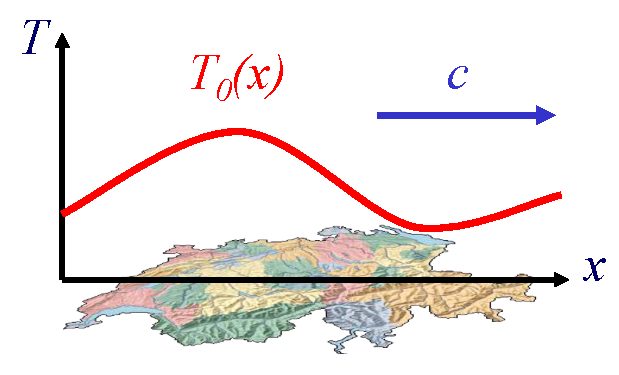
\includegraphics[width=0.45\textwidth]{img/03_weather}
\end{figure}
Given the temperature distribution $T_0(x)$ at time $t=0$ and wind speed $c$. Find an expression for the temperature evolution $T(x,t)$!

\subsection{Analytical Solution}

How does the temperature change over a time interval $\Delta  t$?
\begin{figure}[H]
	\centering
	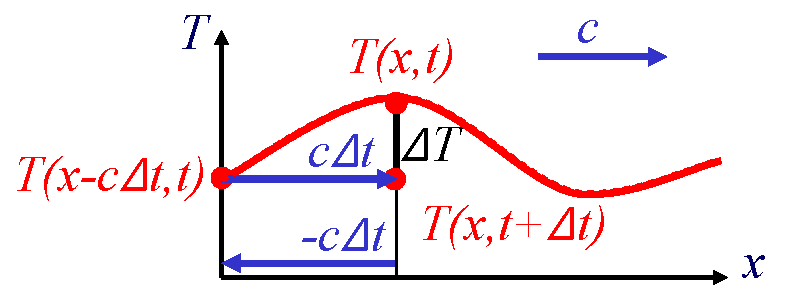
\includegraphics[width=0.45\textwidth]{img/03_1D_advection}
\end{figure}
\begin{align*}
	T(x, t+\Delta t) &= T(x-c\Delta t, t) \\
	\Delta T &= T(x,t+\Delta t) - T(x,t)\\
	T(x-c\Delta t, t) &= T(x,t) - {\partial T \over \partial x} c \Delta t + \bigO{\Delta t^2} = T(x, t+\Delta t)
\end{align*}

From which we can build the advection equation:
\begin{align*}
	{\Delta T  \over \Delta} t \approx -c {\partial T \over \partial x} \quad
	\lim_{\Delta \mapsto 0} \implies \quad {\partial T \over \partial t} = -c {\partial T \over \partial x}
\end{align*}
Any $T(x,t)$ of the form $T(x,t) = f(x-ct)$ solves ${\partial T \over \partial t} = -c {\partial T \over \partial x}$.  The solution also needs to satisfy the initial condition:
	\begin{align*}
		T(x,0) &= T_0(x)
	\end{align*}
	The solution is thus
	\begin{align*}
		T(x, t) &= T_0(x-ct)
	\end{align*}

\subsection{Numerical Solution}
Sample temperature $T(x,t)$ on 1D grid $T^t[i] = T(i\cdot h, t\cdot \Delta t)$ with $i \in (1,\ldots n)$, $t \in (0,1,2, \ldots)$:
\begin{figure}[H]
	\centering
	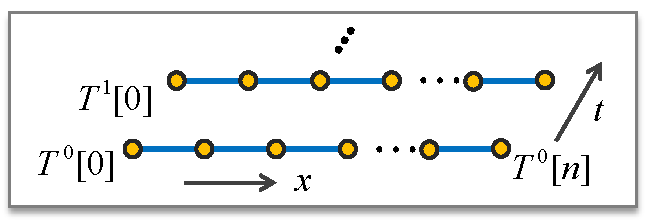
\includegraphics[width=0.45\textwidth]{img/03_numerical_solution}
	\caption{Sampling Grid}
\end{figure}

\section{Overview}
\begin{description}
	\item[Order of PDE] The \emph{order} of a PDE is the order of it's highest partial derivative.
	\item[Linearity] A PDE is \emph{linear} if the unknown function $(u)$ and it's partial derivatives only occure linearly:
		\begin{align*}
			\text{Linear example: }\ & u_t+c\cdot u_x = 0 & \text{(Advection eq.)}\\
			\text{Nonlinear example: }\ & u_t+u\cdot u = 0 & \text{(Burger's eq.)}
		\end{align*}
		Coefficients of linear PDEs can be nonlinear functions:
		\begin{align*}
			y^2 \cdot u_{yy} + x^2 \cdot u_{yy} = 0
		\end{align*}


\end{description}

\subsection{PDE Classification}
$2^{nd}$ order linear PDEs are of highest practical relevance. A $2^{nd}$ order linear PDE has the form:
\begin{align*}
	Au_{xx} + 2Bu_{xy} + Cu_{yy} = F(x,y,u, u_x, u_y).
\end{align*}
A $2^{nd}$ order linear PDE is either:
\begin{align*}
	\textbf{Hyperbolic}\quad B^2-AC > 0 &\text{Wave equation}\\
	\textbf{Parabolic}\quad B^2-AC = 0 &\text{Heat equation}\\
	\textbf{Elliptic}\quad B^2-AC < 0 &\text{Laplace equation}
\end{align*}

\begin{figure}[H]
	\centering
	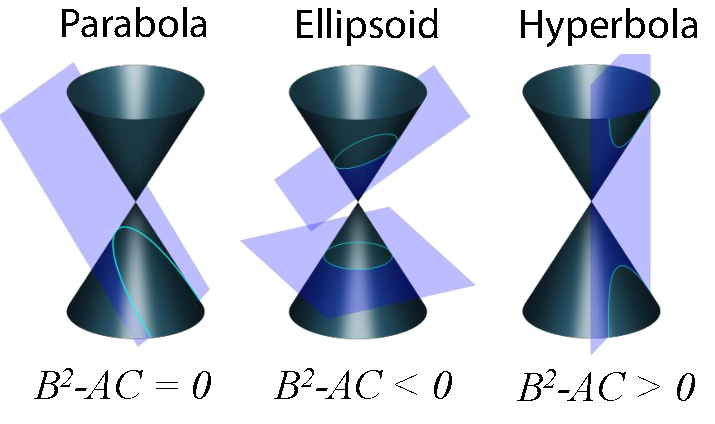
\includegraphics[width=0.45\textwidth]{img/03_PDE_classification}
\end{figure}

\subsection{Hyperbolic PDEs}
Hyperbolic PDEs are typically time dependent problems. They retain \& propagate disturbances present in initial data.
\paragraph{Prototype:} let $u$ be the amplitude and $c$ the propagation speed:
\begin{align*}
	\textbf{\emph{Wave Equation}:}\quad {\partial^2 u \over \partial t^2} = {\partial^2 u \over \partial x^2} c^2
\end{align*}
\paragraph{Applications}
\begin{itemize}
	\item Simulate wave propagation for sound, light and water.
	\item Mechanics: Oscillatory motion, vibrating strings.
\end{itemize}

\subsection{Parabolic PDEs}
Parabolic PDEs are typically time dependent problems. Solutions \emph{smooth out} as time increases.
\paragraph{Prototype:} let $u$ be the temperature and $\alpha$ the thermal diffusivity:
\begin{align*}
	\textbf{\emph{Heat Equation}:}\quad {\partial u \over \partial t} = \alpha {\partial^2 u \over \partial x^2}
\end{align*}

\paragraph{Application} consist of conduction and general diffusion processes.

\subsection{Elliptic PDEs}
Elliptic PDEs describe static problems (i.e. systems in equilibrium). Solutions are smooth (if the coefficients are).
\paragraph{Prototype:} 
\begin{align*}
	\textbf{\emph{Laplace Equation}:}\quad {\partial^2 u \over \partial x^2} + {\partial^2 u \over \partial y^2} = 0
\end{align*}

\paragraph{Applications} consist of steady-state solutions to hyperbolic and parabolic PDEs and of equilibrium problems.

\section{Boundary Conditions}
Generally there are (infinitely) many $u$ which solve a PDE. So there's additional information required $\rightarrow$ \emph{Boundary Conditions}. Typically $u$ is defined in a region $D$ and the solution is required to satisfy certain conditions on the boundary $\delta D$ of $D$:
\begin{figure}[H]
	\centering
	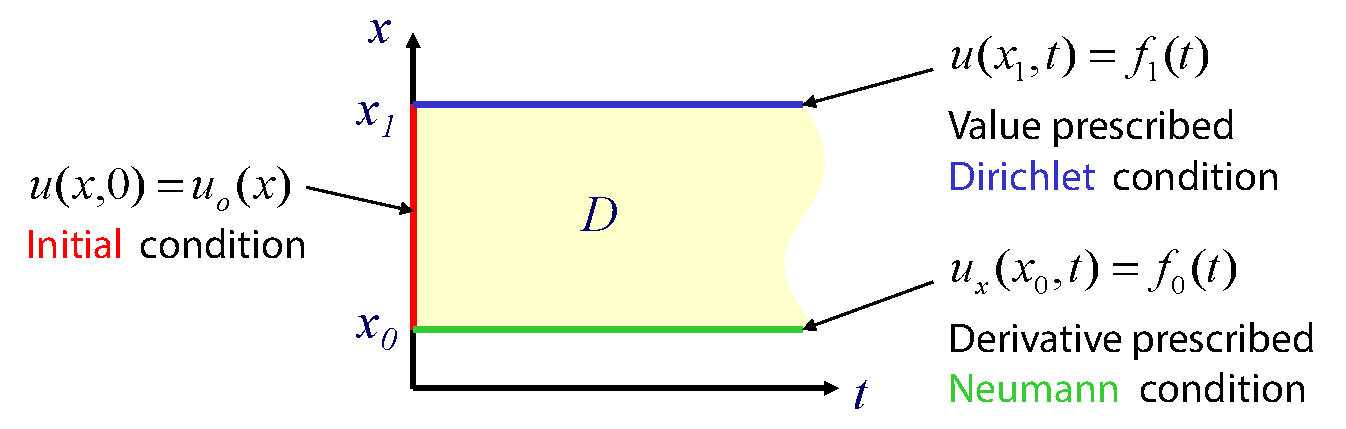
\includegraphics[width=0.45\textwidth]{img/03_boundary_conditions}
\end{figure}







\end{multicols}